\documentclass{standalone}
\usepackage{tikz}
\usepackage{hyperref}
\usetikzlibrary{
  arrows,
  calc,
  decorations.pathmorphing,
  decorations.pathreplacing,
  decorations.markings,
  positioning,
  shapes,
  arrows.meta
}

\ifpdf
% Ensure reproducible output
\pdfinfoomitdate=1
\pdfsuppressptexinfo=-1
\pdftrailerid{}
\hypersetup{
  pdfcreator={},
  pdfproducer={}
}
\fi

\begin{document}

\begin{tikzpicture}
  \node at (-5, 0) {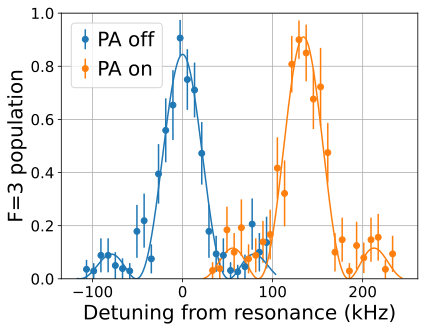
\includegraphics[height=3.8cm]{pa_vectorshift_spectrum.pdf}};
  \node at (-2.95, 1.5) {\footnotesize (\textbf{A})};
  \node at (0.2, -0.045) {\includegraphics[height=3.8cm]{pa_vectorshift_align.pdf}};
  \node at (2.25, 1.5) {\footnotesize (\textbf{B})};
\end{tikzpicture}

\end{document}
